\section{Cálculos de la estructura}
\label{Ap:Estructura}

\begin{center}
    $\tau=FdSin\theta$
\end{center}

Si el ángulo $\theta$ se considera máximo, al aplicar la carga con un ángulo de $90 ^oC$ se tiene.

Donde: \\
$F$ es el peso de la materia orgánica en $[N]$\\
$d$ es la distancia del eje de rotación al extremo de la pala en $[m]$\\
$\theta$ es el ángulo de aplicación de la fuerza en $[^oC]$

\section{Potencia Consumida}\label{Ap:Eje}

\begin{center}
  $\omega = \frac{\theta}{t} $  
\end{center}
Selección
Donde: \\
$\theta$ son las vueltas en radianes \\
$t$ es el tiempo en segundos


\begin{center}
 $P_{cons}=M_t * \omega$   
\end{center}

Donde: \\

$M_t$ es el Momento de torsión $\tau$ \\
$\omega$ es la velocidad angular previamente calculada
\newpage

\section{Diseño de la transmisión por bandas}\label{Ap:Eje }

\begin{figure}[h]
    \centering
        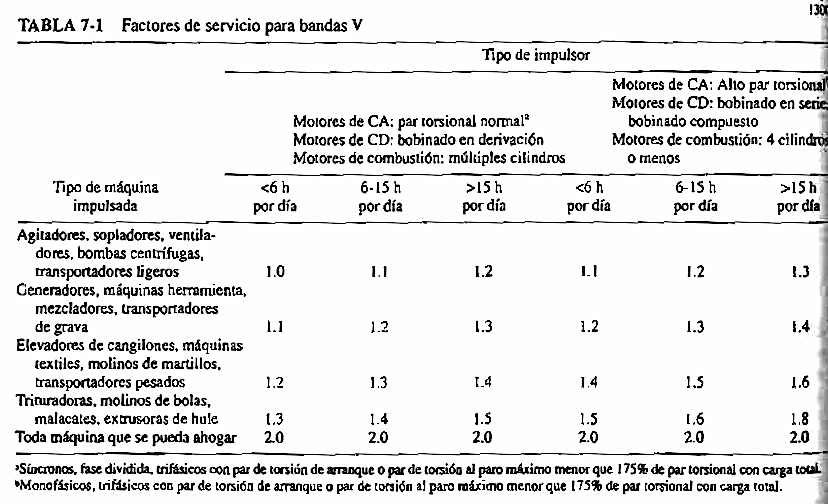
\includegraphics[scale=0.8]{images/Capitulo 4/s5/Factores de servicio.png}
        \caption{Factores de Servicio para bandas V}\cite{Mott}
    \label{fg:Factores}
\end{figure}

\begin{figure}[h]
    \centering
        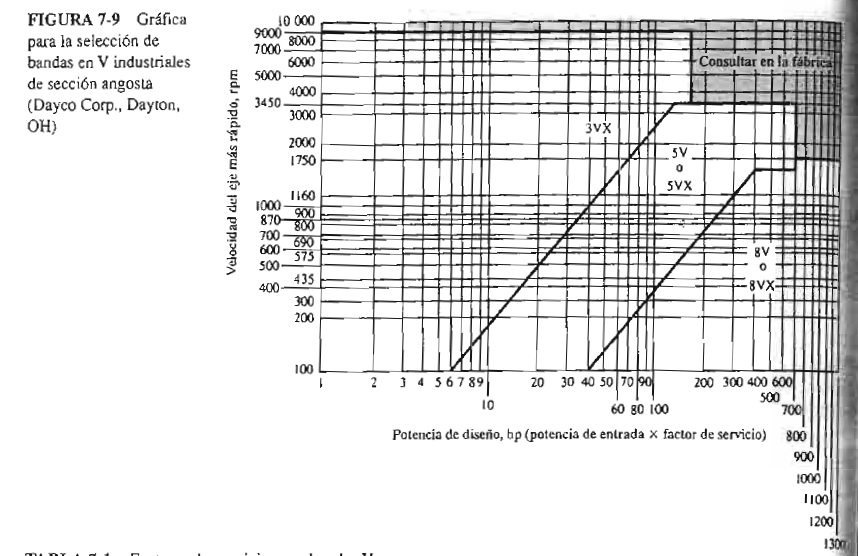
\includegraphics[scale=0.7]{images/Capitulo 4/s5/Grafica para la seleccion de bandas.png}
        \caption{Gráfica para la selección de bandas}\cite{Mott}
    \label{fg:Bandas}
\end{figure}

\begin{figure}[h]
    \centering
        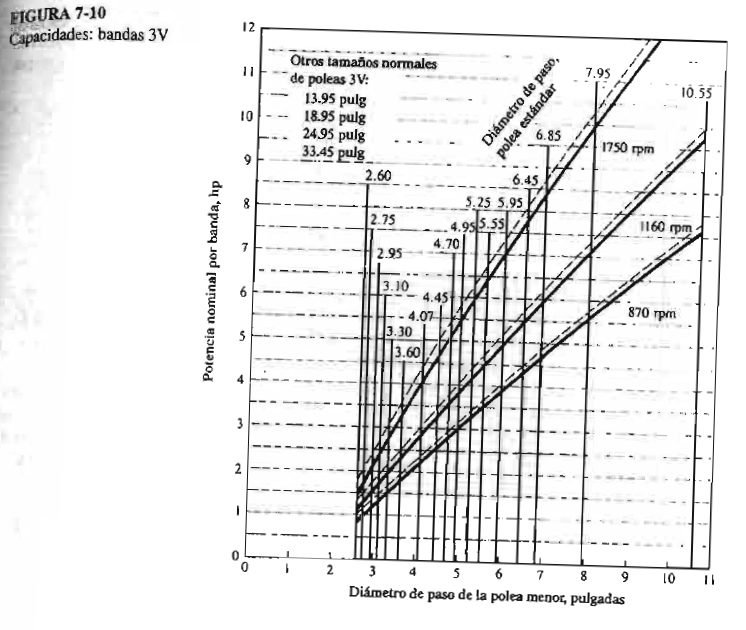
\includegraphics[scale=1]{images/Capitulo 4/s5/Capacidad 3V.png}
        \caption{Capacidad Banda 3V}\cite{Mott}
    \label{fg:Banda3V}
\end{figure}

\begin{figure}[h!]
    \centering
        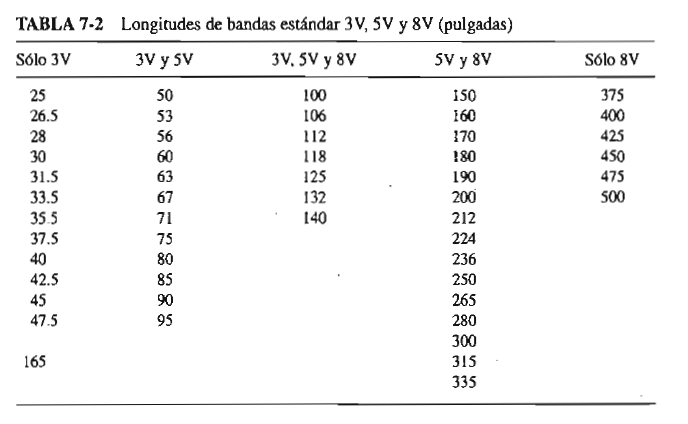
\includegraphics[scale=1.1]{images/Capitulo 4/s5/Longitudes bandas.png}
        \caption{Longitudes de Bandas estándar}\cite{Mott}
    \label{fg:Longitud}
\end{figure}
\newpage

\begin{figure}[h!]
    \centering
        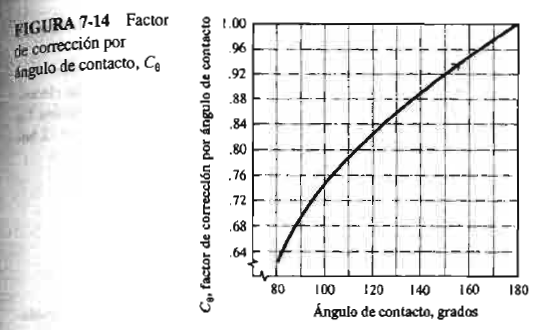
\includegraphics[scale=1]{images/Capitulo 4/s5/Factor theta.png}
        \caption{Factor theta}\cite{Mott}
    \label{fg:theta}
\end{figure}
\begin{figure}[h!]
    \centering
        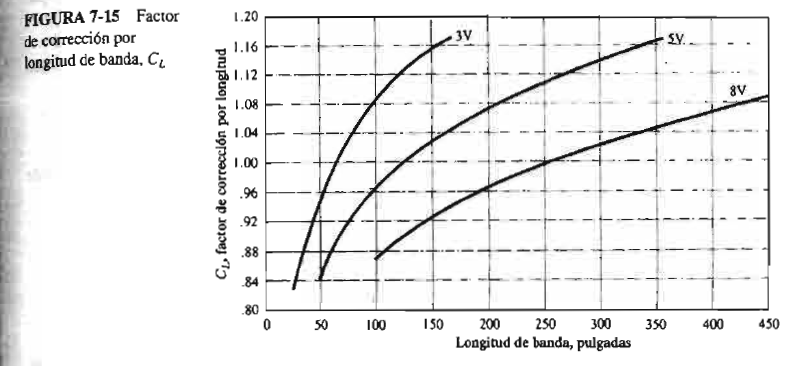
\includegraphics[scale=0.9]{images/Capitulo 4/s5/Factor L.png}
        \caption{Factor Longitud}\cite{Mott}
    \label{fg:L}
\end{figure}
\newpage


\section{Diseño de la cuña}
\label{Ap:Eje Seleccion}
\begin{figure}[h!]
    \centering
        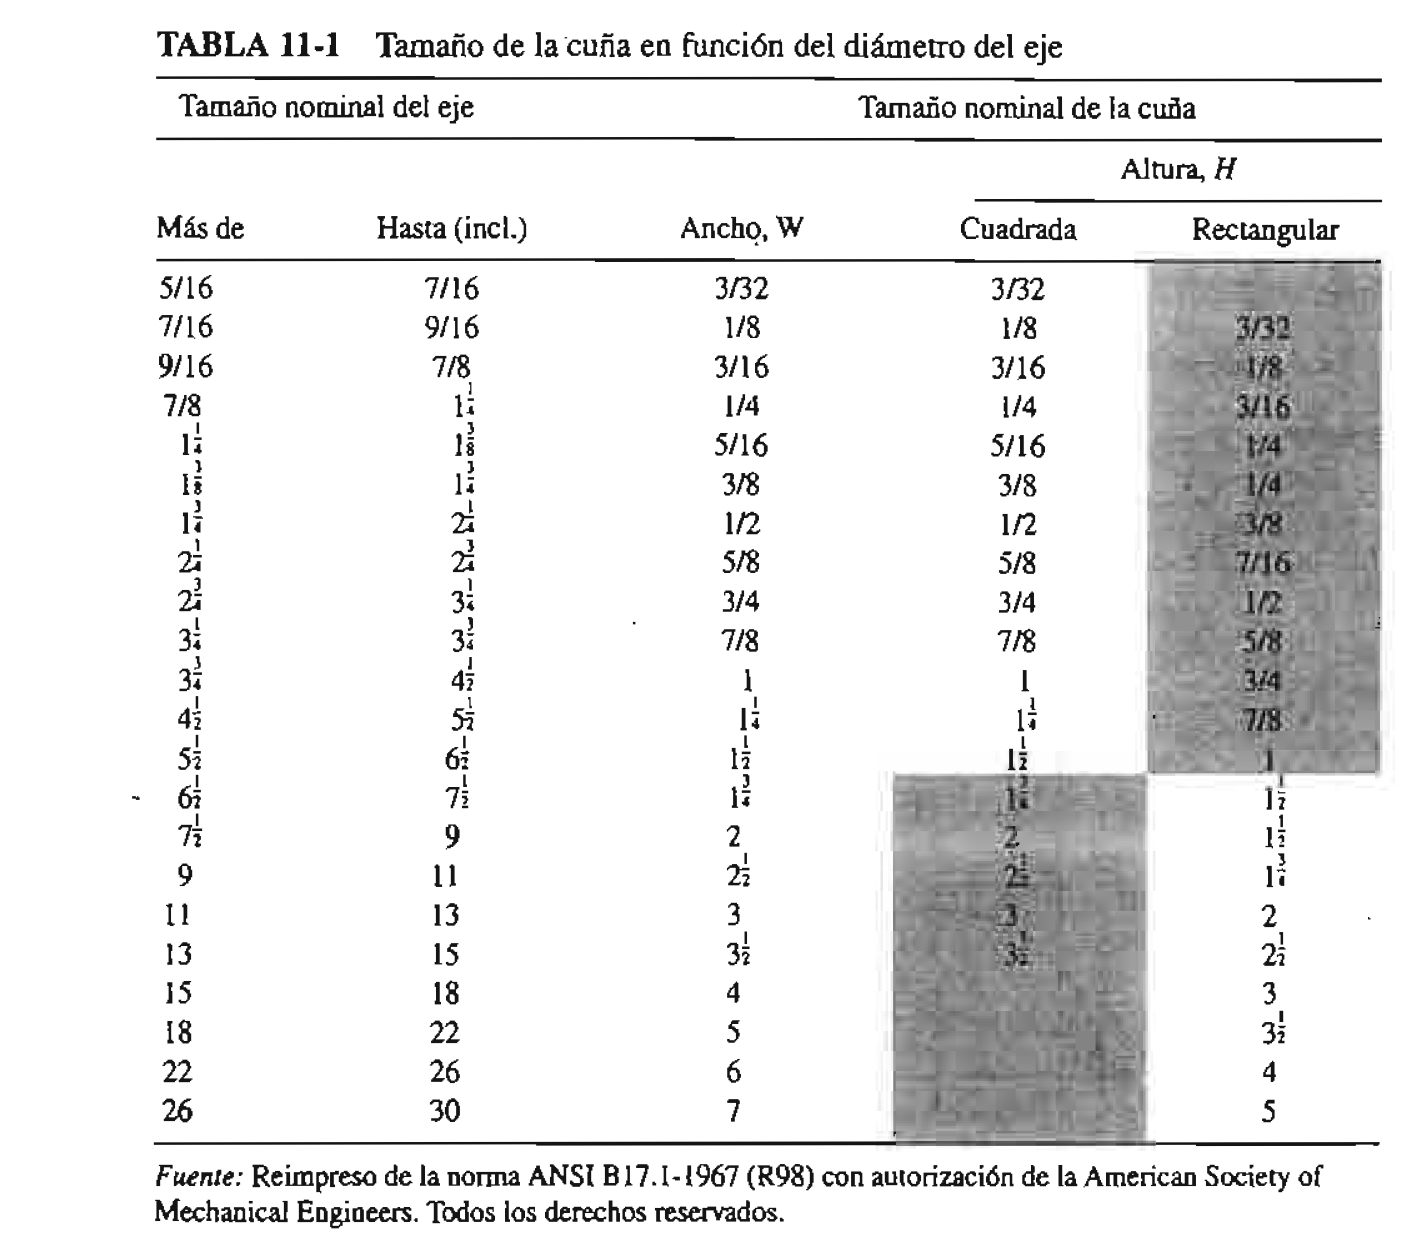
\includegraphics[scale=0.5]{images/Capitulo 4/s5/Tamanos Cuna.png}
        \caption{Tamaño de cuña en función del diámetro del eje }\cite{Mott}
    \label{fg:Tamaños Cuña}
\end{figure}
\newpage

\section{Diseño del eje de Aireación}\label{Ap:Eje Seleccion}
\begin{center}
    $D=\sqrt[3]{\frac{32*N}{\pi}*\sqrt{(K_t*\frac{M}{s'n})^2+ \frac{3}{4}*(\frac{T}{S_y})^2}}$
\end{center}

Donde: \\
$K_t$ es la concentración de esfuerzos que se producen por variaciones geométricas. \\
$N$ Factor de diseño.\\
$s'n$ es el valor de la resistencia a la fatiga según el material seleccionado.\\
$M$ momentos flexionantes. \\
$T$ es el torque al que se ve sometido el eje. \\
$S_y$ esfuerzo de fluencia.

\begin{center}
    $s'n =  sn*C_m*C_{st}*C_r*C_s$
\end{center}

Donde: \\
s’n: valor de la resistencia real a la fatiga. \\
sn: es el valor de resistencia a la fatiga teórico. \\
$C_m$: factor de material. \\
$C_{st}$: factor de tipo de esfuerzo. \\
$C_r$: factor de confiabilidad \\
$C_s$: factor de tamaño \\

\begin{figure}[h]
    \centering
        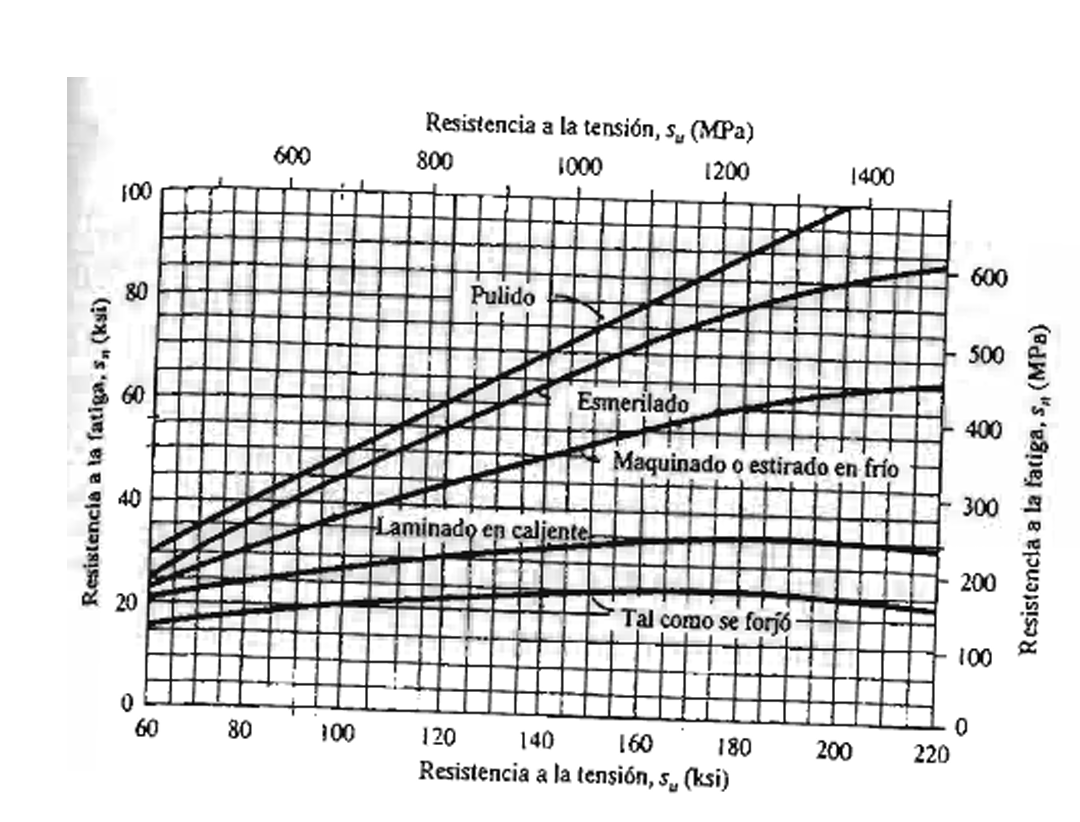
\includegraphics[scale=0.6]{images/Capitulo 4/s5/Resistencia a la fatiga.png}
        \caption{Resistencia a la fatiga}\cite{Mott}
    \label{fg:Res_fat}
\end{figure}
\begin{figure}[p]
    \centering
        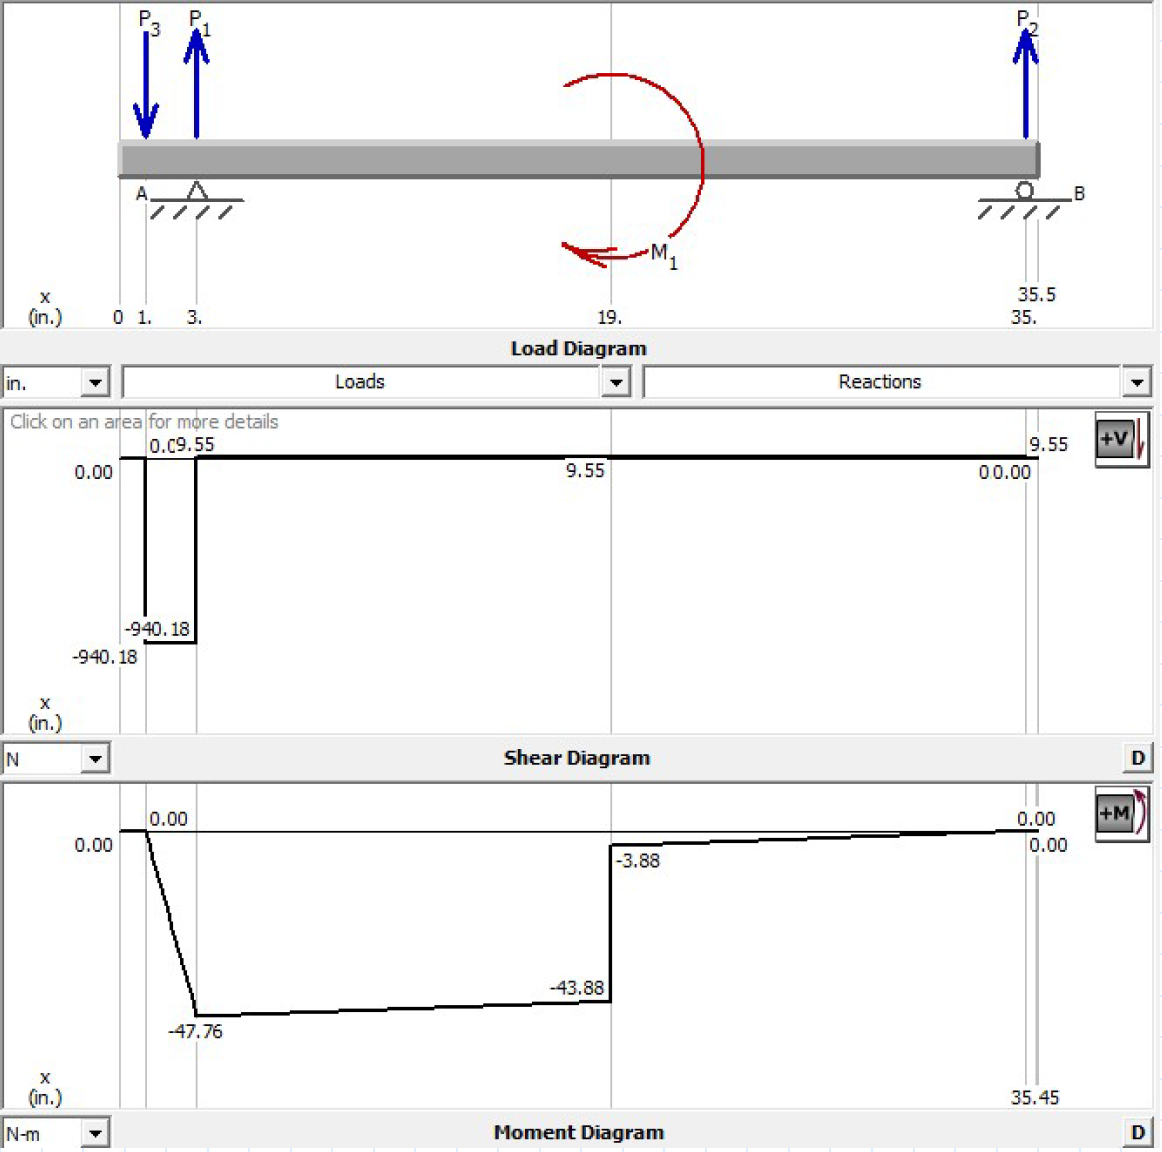
\includegraphics[scale=0.8]{images/Capitulo 4/s5/1 pala fuerzas.png}
        \caption{Fuerzas, Esfuerzos y Momentos del lado del eje con 1 pala}
    \label{fg:1palaF}
\end{figure}
\begin{figure}[p]
    \centering
        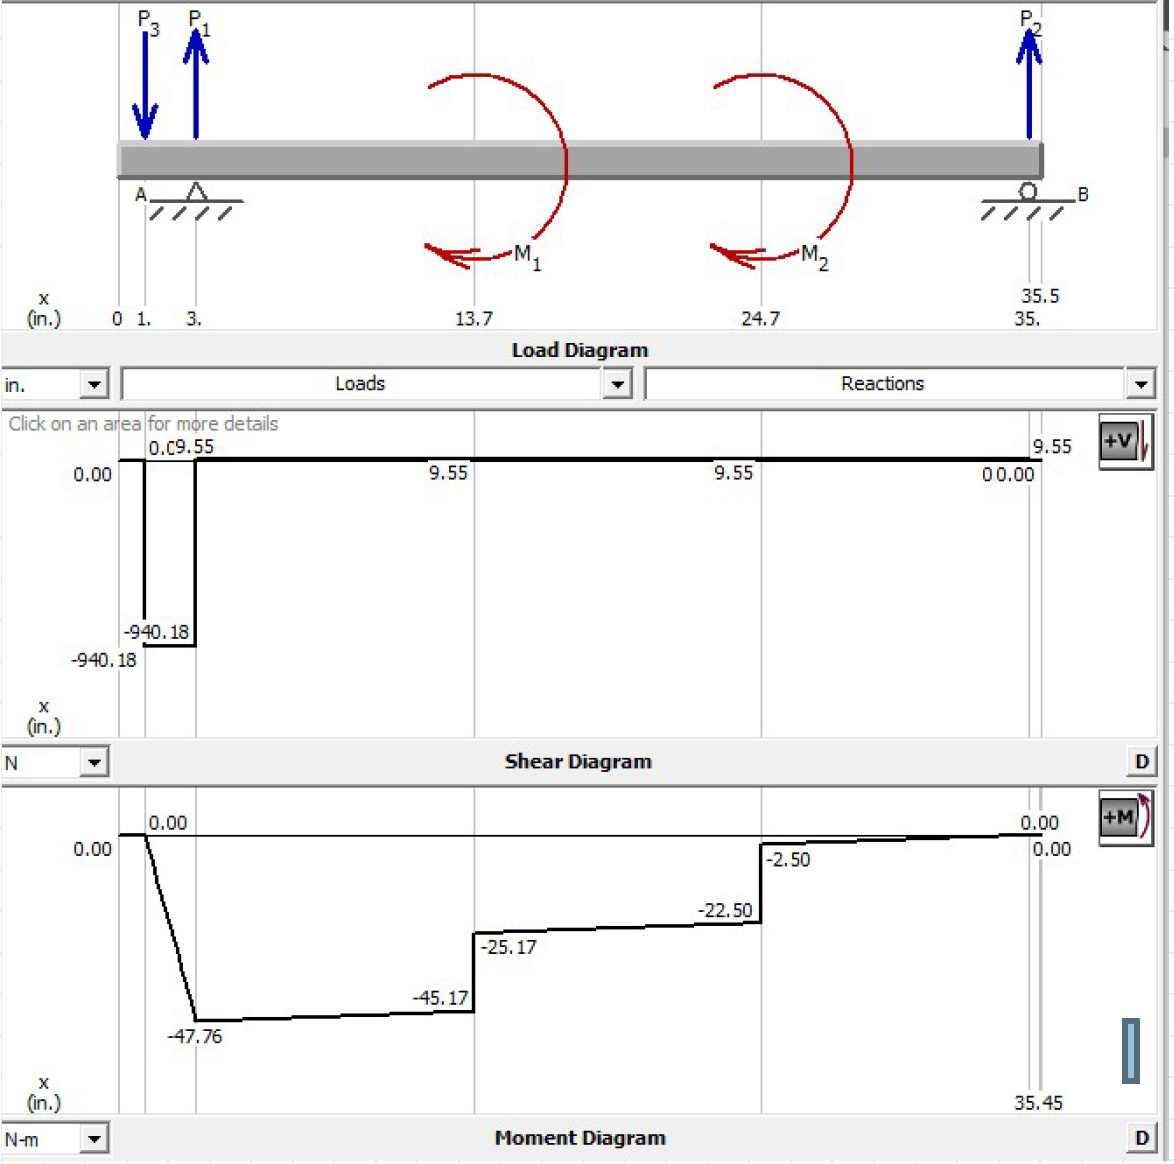
\includegraphics[scale=0.8]{images/Capitulo 4/s5/2 palas fuerzas.png}
        \caption{Fuerzas, Esfuerzos y Momentos del lado del eje con 2 palas}
    \label{fg:2palasF}
\end{figure}